\chapter*{}
Personalmente, este proyecto ha sido una oportunidad para profundizar en tecnologías y conceptos que no formaban parte de mi conocimiento previo. Desde el aprendizaje de nuevas herramientas como Spring Boot y Maven hasta la adopción de buenas prácticas como la documentación con Javadoc y el uso de estándares de Java, he adquirido habilidades que serán valiosas en futuros proyectos. Además, la experiencia de trabajar en un proyecto de esta envergadura ha reforzado mi capacidad para planificar, organizar y resolver problemas de manera eficiente.

En conclusión, este proyecto no solo ha cumplido con sus objetivos iniciales, sino que también ha sentado las bases para futuras mejoras y desarrollos. Espero que el trabajo realizado contribuya al avance de aplicaciones similares y sirva como referencia para otros desarrolladores e investigadores.

%%\nocite{*} %incluye TODOS los documentos de la base de datos bibliográfica sean o no citados en el texto
\newpage
\printbibliography

%\bibliography{bibliografia/bibliografia}
%\addcontentsline{toc}{chapter}{Bibliografía} %sustituir bibliografía con el nombre del fichero bibtex con la bibliografía
%


\appendix
\chapter{Anexo I. Esquema de base de datos}


\begin{figure}
    \centering
    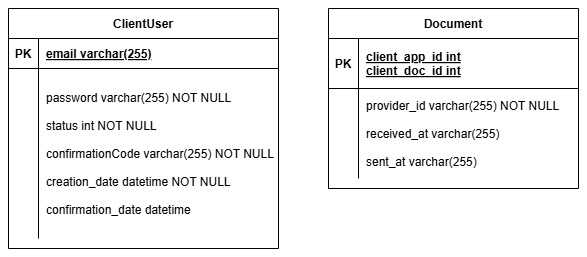
\includegraphics[width=0.5\linewidth]{imagenes//scheme/SIDManager_BD.jpg}
    \caption{Esquema de  la base de datos}
    \label{fig:BD-scheme}
\end{figure}

\chapter{Anexo II. Código de la aplicación SIDManager}

\begin{lstlisting}[
    language=xml,
    label=code:kachiquel_xml,
    caption={Kaqchikel XML generado por el LLM a partir de la imagen de la página original}
]
<?xml version="1.0" encoding="UTF-8"?>
<document>
    <page number="203">
        <heading>... / .. / .... Oración compleja</heading>
        <line>La oración compleja se forma con más de una cláusula, una de ellas es la principal y</line>
        <line>otra la subordinada. La idea que expresan las cláusulas subordinadas siempre dependen</line>
        <line>de la cláusula principal, su posición es siempre después de ésta. Una cláusula subordinada</line>
        <line>se introduce por medio de subordinadores, aunque hay excepciones. Son oraciones</line>
        <line>complejas si dentro de la cláusula principal se encuentran las siguientes cláusulas</line>
        <line>subordinadas:</line>
       
        <line>Cláusula relativa</line>
        <line>Cláusula adjunta o adverbial</line>
        <line>Cláusula de complemento</line>


        <heading>... / .. / .... / . Clausula relativa</heading>
        <line>La clausula relativa modifica a sustantivos, describe alguna caracteristica, por eso</line>
        <line>funciona como adjetivo. La clausula relativa se introduce por los subordinadores: ri,</line>
        <line>re, la, achoq rik'in y achoq chi re o simplemente subordinador. Estas particulas se</line>
        <line>conocen con los nombres de pronombre relativo o relativizador. Si modifica al sujeto u</line>
        <line>objeto, se introduce con las particulas: ri, re, la. Si modifica al instrumento o compania,</line>
        <line>la clausula relativa se introducen con la frase achoq rik'in; y si la clausula no se</line>
        <line>introduce por subordinador, la clausula relativa se escribe entre comas. Ejemplos:</line>


        <line>Modificando al sujeto:</line>
        <interlinear_gloss>
            <parallel_phrase>
                <original>Ri ix\"{o}q, ri xkos, xb'eruloq'o' xkoya'.</original>
                <translation>La mujer que se cansó fue a comprar tomate</translation>
            </parallel_phrase>
            <morpheme_analysis>
                <unit>
                    <form>Ri</form>
                    <gloss>DET</gloss>
                </unit>
                <unit>
                    <form>ix\"{o}q,</form>
                    <gloss>mujer</gloss>
                </unit>
                <unit>
                    <form>ri</form>
                    <gloss>CR</gloss>
                </unit>
                <unit>
                    <form>x-</form>
                    <gloss>COM-</gloss>
                </unit>
                <unit>
                    <form>{\O}-</form>
                    <gloss>B3s-</gloss>
                </unit>
                <unit>
                    <form>kos,</form>
                    <gloss>cansar</gloss>
                </unit>
                <unit>
                    <form>x-</form>
                    <gloss>COM-</gloss>
                </unit>
                <unit>
                    <form>{\O}-</form>
                    <gloss>B3s-</gloss>
                </unit>
                <unit>
                    <form>b'e-</form>
                    <gloss>MOV-</gloss>
                </unit>
                <unit>
                    <form>ru-</form>
                    <gloss>A3s-</gloss>
                </unit>
                <unit>
                    <form>loq'-</form>
                    <gloss>comprar-</gloss>
                </unit>
                <unit>
                    <form>o'</form>
                    <gloss>SC</gloss>
                </unit>
                <unit>
                    <form>xkoya'.</form>
                    <gloss>tomate</gloss>
                </unit>
            </morpheme_analysis>
            <syntactic_analysis>
                <unit>
                    <form>ri xkos</form>
                    <gloss>CR</gloss>
                </unit>
            </syntactic_analysis>
        </interlinear_gloss>


        <interlinear_gloss>
            <parallel_phrase>
                <original>Re ak'wal, re xtzaq, xoq'.</original>
                <translation>Este niño que se cayó, lloró.</translation>
            </parallel_phrase>
            <morpheme_analysis>
                <unit>
                    <form>Re</form>
                    <gloss>DET</gloss>
                </unit>
                <unit>
                    <form>ak'wal,</form>
                    <gloss>niño,</gloss>
                </unit>
                <unit>
                    <form>re</form>
                    <gloss>CR</gloss>
                </unit>
                <unit>
                    <form>x-</form>
                    <gloss>COM-</gloss>
                </unit>
                <unit>
                    <form>{\O}-</form>
                    <gloss>B3s-</gloss>
                </unit>
                <unit>
                    <form>tzaq,</form>
                    <gloss>caer</gloss>
                </unit>
                <unit>
                    <form>xoq'.</form>
                    <gloss>llorar</gloss>
                </unit>
            </morpheme_analysis>
            <syntactic_analysis>
                <unit>
                    <form>re xtzaq</form>
                    <gloss>CR</gloss>
                </unit>
            </syntactic_analysis>
        </interlinear_gloss>


        <interlinear_gloss>
            <parallel_phrase>
                <original>La k'aj\"{o}l, la xloq'o ri wexaj, xb'e.</original>
                <translation>Ese muchacho que compr\'o el pantal\'on, se fue.</translation>
            </parallel_phrase>
            <syntactic_analysis>
                <unit>
                    <form>la xloq'o ri wexaj</form>
                    <gloss>CR</gloss>
                </unit>
            </syntactic_analysis>
        </interlinear_gloss>
    </page>
</document>

}
\end{lstlisting}

\begin{lstlisting}[
    language=Java, 
    label=code:not-received-controller, 
    caption={Función getNotReceivedDocuments del controlador}
]
@GetMapping ("/not-received")
public String getNotReceivedDocuments(Model model){
    logger.debug(" ----- Entering getNotReceivedDocuments ----- " );
    model.addAttribute("documents" , documentService.getNotReceivedDocuments());
    model.addAttribute ("isShowingUnsaveds", "Yes");
    logger.debug(" ----- Exiting getNotReceivedDocuments ----- ");
    return "documentsView";
}
\end{lstlisting}



\begin{lstlisting}[
    language=Java,
    label={code:not-received-service},
    caption={Función getNotReceivedDocuments del servicio}
]
public List<Document> getNotReceivedDocuments() {
    logger.debug(" Entering getNotReceivedDocuments ");
    return documentRepository.findByReceivedAtIsNull();
}
\end{lstlisting}



\begin{lstlisting}[
    language=Java, 
    label=code:list-docs,
    caption={Función listDocuments del controlador}
]
@GetMapping("/list")
public String listDocuments(
        @RequestParam(value = "min-date",  required = false) String startDate,
        @RequestParam(value = "max-date", required = false) String endDate,
        Model model) throws Exception {
    logger.debug(" ----- Entering listDocuments ----- ");
    
    DateRange dateRange = documentService.checkDates(startDate, endDate, model);
    
    model.addAttribute("documents", 
            documentService.getFilteredDocuments(
                    dateRange.getStartDate(),
                    dateRange.getEndDate()
                    ));    	
    model.addAttribute("startDate", dateRange.getStartDate());
    model.addAttribute("endDate", dateRange.getEndDate());
    model.addAttribute("isShowingUnsaveds", "No");
    
    logger.debug(" ----- Exiting listDocuments ----- ");
    logger.debug(" ____________________________________ ");
        
    return "documentsView";
}
\end{lstlisting}



\begin{lstlisting}[
    language=Java, 
    label=code:list-docs-service,
    caption={Función getFilteredDocuments del servicio}
]
public List<Document> getFilteredDocuments(Date startDate, Date endDate) {
    logger.debug(" Entering getFilteredDocuments ");
    return documentRepository.findFilteredDocuments(startDate, endDate);
}
\end{lstlisting}



\begin{lstlisting}[
    language=Java,
    label=code:list-docs-repositoty,
    caption={Función findFilteredDocuments del repositorio}
]
@Query(value = "SELECT CLIENT_APP_ID, CLIENT_DOC_ID, PROVIDER_ID, SENT_AT, RECEIVED_AT"
            + " FROM documents WHERE SENT_AT > :startDate AND SENT_AT < :endDate", nativeQuery = true)
List<Document> findFilteredDocuments(@Param("startDate") Date startDate, @Param("endDate") Date endDate); 
\end{lstlisting}



\begin{lstlisting}[
    language=Java, 
    label={code:checkDates},
    caption={Función checkDates del servicio}
]
public DateRange checkDates(String stringStartDate, String stringEndDate, Model model) {
    final int daysRange = 10;  
    DateRange dateRange;
    boolean isCorrectRange = true;
    
    try {
        if (DateUtils.checkDate(stringStartDate) && DateUtils.checkDate(stringEndDate)) {
            Date startDate = DateUtils.stringToUtilsDate(stringStartDate);
            Date endDate = DateUtils.stringToUtilsDate(stringEndDate);
            
            int daysBetween = DateUtils.daysBetween(startDate, endDate);
            
            if(daysBetween != -1 && daysBetween <= daysRange) {
                dateRange = new DateRange(startDate, endDate);
                logger.info(" Returning FILTERED documents ");
            } else {
                dateRange = new DateRange(-daysRange);
                
                logger.warn(" Exceded maximum day range ( " +
                            daysBetween + 
                            " ) with: " + 
                            daysRange);
                logger.warn(" Returning last 10 days ");
                
                isCorrectRange = false;
            }
        } else if (DateUtils.checkDate(stringEndDate)) {
            dateRange = new DateRange(DateUtils.stringToUtilsDate(stringEndDate), -daysRange);
            isCorrectRange = false;
        } else if (DateUtils.checkDate(stringStartDate)) {
            dateRange = new DateRange(DateUtils.stringToUtilsDate(stringStartDate), daysRange);
            isCorrectRange = false;
        } else {
            dateRange = new DateRange(-daysRange);
        }
    } catch (ParseException e) {
        logger.error(" ERROR in getFilteredDocuments: " + e);
        dateRange = new DateRange(-daysRange);			
    }
    
    if (!isCorrectRange) {
        model.addAttribute("responseMessage", ResponseEnum.LIST_WARNING_1.getMessageKey());
        model.addAttribute("isAWarningMessage", true);
    }
    
    return dateRange;
}
\end{lstlisting}



\begin{lstlisting}[
    language=Java, 
    label=code:getCreateClientUserView,
    caption={Función getCreateClientUserView del controlador}
]
@GetMapping("/user/create")
public String getCreateClientUserView() {
    logger.debug("Entering GET: /user/create");
    
    return "createClientUserView"; 
}
\end{lstlisting}



\begin{lstlisting}[
    language=Java,
    label=code:createClientUser-controller,
    caption={Función createClientUser del controlador}
]
@PostMapping("/user/create")
public String createClientUser(Model model, 
                                @ModelAttribute ClientUser clientUser,
                                @RequestParam("psw-repeat") String passwordRepeat
                                ) throws Exception {
    
    logger.debug(" - Entering clientUserService.createClientUser(), from POST: /user/create");
    
    ResponseEnum responseMessage = clientUserService.createClientUser(clientUser, passwordRepeat);

    model.addAttribute("responseMessage", responseMessage.getMessageKey());
    addColorToResponse(model, responseMessage);
    
    return "createClientUserView";  
}
\end{lstlisting}



\begin{lstlisting}[
    language=Java,
    label=code:saveClientUser-controller,
    caption={Función saveClientUser del controlador}
]
@Transactional
public ClientUser saveClientUser(ClientUser clientUser) throws Exception {
    try {
        if (clientUser.getPassword() != null) {
            logger.debug(" -- Entering encryptMessage()");
            clientUser.setPassword(encryptFacade(clientUser.getPassword()));
            
            logger.debug(" -- Entering randomAlphanumeric()");
            clientUser.setConfirmationCode(RandomStringUtils.randomAlphanumeric(30));
            
            clientUser.setStatus(0);
            clientUser.setCreationDate(new Date()); 
            clientUserRepository.save(clientUser);
        } else {
             throw new IllegalArgumentException("Password cannot be null");
        }
    } catch (Exception e) {
        logger.error(" ERROR: Possible error in encryption, confirmation code generation "
                + " or saveClientUser:" + e);
        throw e;
    }
    
    return clientUser;
}
\end{lstlisting}



\begin{lstlisting}[
    language=Java,
    label=code:getConfirmation-controller,
    caption={Función getConfirmation del controlador}
]
@GetMapping("/user/confirm")
public String getConfirmation(Model model, 
                              @RequestParam("email") String email,
                              @RequestParam("confirmationCode") String confirmationCode) {
    
    logger.debug(" - Entering clientUserService.confirmUser(), from GET: /user/confirm");
    ResponseEnum responseMessage = clientUserService.confirmUser(email, confirmationCode);
    logger.debug(" - Exiting clientUserService.confirmUser()");
    
    model.addAttribute("responseMessage", responseMessage.getMessageKey());
    addColorToResponse(model, responseMessage);
    
    return "confirmationUser"; 
}    
\end{lstlisting}


\begin{lstlisting}[
    language=Java,
    label=code:confirmUser-service,
    caption={Función confirmUser del servicio}
]
@Transactional
public ResponseEnum confirmUser(String email,
                                String confirmationCode
                                ) {
    ResponseEnum responseMessage;
    ClientUser clientUser = clientUserRepository.findByEmailAndConfirmationCodeAndStatus(email, confirmationCode, 0);	
    
    if (clientUser != null) {
        responseMessage = ResponseEnum.CONFIRM_SUCCESS;
        clientUser.setStatus(1);
        clientUser.setConfirmationDate(new Date()); 
        clientUserRepository.save(clientUser);
    } else {
        logger.debug(" User not found, not correct or already confirmed. ");
        responseMessage = ResponseEnum.CONFIRM_WARNING;
    }
    
    return responseMessage;
}
\end{lstlisting}


\begin{lstlisting}[
    language=Java,
    label=code:getLoginView-controller,
    caption={Función getLoginView del controlador}
]
@GetMapping("/user/login")
public String getLoginView(Model model,
                           HttpServletRequest request
                           ) throws Exception {
    String serverUrl = SharedProperties.get("serverUrl");
    String requestUpdatePasswordUrl =  serverUrl + "user/requestUpdatePassword";
    String createClientUserUrl = serverUrl + "user/create";
    String errorMessage = (String) request.getSession().getAttribute("error");
    
    model.addAttribute("requestUpdatePasswordUrl", requestUpdatePasswordUrl);
    model.addAttribute("createClientUserUrl", createClientUserUrl);
    
    if (errorMessage != null) {
        ResponseEnum responseMessage = ResponseEnum.LOGIN_WARNING_1;
        model.addAttribute("responseMessage", responseMessage.getMessageKey());
        addColorToResponse(model, responseMessage);
        
        // Elimina el mensaje de error de la sesión
        request.getSession().removeAttribute("error");
    }
    
    return "loginView";
}
\end{lstlisting}



\begin{lstlisting}[
    language=Java,
    label=code:getRequestUpdatePasswordView-controller,
    caption={Función getRequestUpdatePasswordView del controlador}
]
@GetMapping("/user/requestUpdatePassword")
public String getRequestUpdatePasswordView() {
    return "requestUpdatePasswordView";
}
\end{lstlisting}



\begin{lstlisting}[
    language=Java,
    label=code:requestUpdatePassword-controller,
    caption={Función requestUpdatePassword del controlador}
]
@PostMapping("user/requestUpdatePassword")
public String requestUpdatePassword(Model model,
        @RequestParam("email") String email
        ) throws Exception  {
    
    ResponseEnum responseMessage = clientUserService.sendUpdatePasswordUrl(email);
    
    model.addAttribute("responseMessage", responseMessage.getMessageKey());
    addColorToResponse(model, responseMessage);
    
    return "requestUpdatePasswordView";
}
\end{lstlisting}




\begin{lstlisting}[
    language=Java,
    label=code:sendUpdatePasswordUrl-service,
    caption={Función sendUpdatePasswordUrl del servicio}
]
public ResponseEnum sendUpdatePasswordUrl(String email) throws Exception {
    ResponseEnum responseMessage;
    ClientUser clientUser = clientUserRepository.findByEmail(email);
    
    if (clientUser != null && clientUser.getStatus() == 1) {
        String path = "user/updatePassword?email=";
        String urlUpdatePassword = this.getConfirmationUrl(clientUser, path);
        
        logger.debug(" - Entering sendMail");
        String subject = " Change the password of your SIDManager user. ";
        String body = " Click on the next URL if you want to change your password: ";
        Mail.sendMail(clientUser.getEmail(), urlUpdatePassword, subject, body);
        logger.debug(" - Exiting sendMail");
        
        responseMessage = ResponseEnum.UPDATE_PSW_SUCCESS_1;
    } else {
        responseMessage = ResponseEnum.UPDATE_PSW_WARNING_1;
        logger.info(" The user does not exist or is not confirmed. ");
    }

    return responseMessage;
}
\end{lstlisting}



\begin{lstlisting}[
    language=Java,
    label=code:getConfirmationUrl-service,
    caption={Función getConfirmationUrl del servicio}
]
private String getConfirmationUrl(ClientUser clientUser,
      String path
      ) throws Exception {
    StringBuilder confirmationUrl = new StringBuilder();
    String serverUrl = SharedProperties.get("serverUrl");
    
    confirmationUrl.append(serverUrl);
    confirmationUrl.append(path);
    confirmationUrl.append(clientUser.getEmail());
    confirmationUrl.append("&confirmationCode=");
    confirmationUrl.append(clientUser.getConfirmationCode());
    
    return confirmationUrl.toString();
}
\end{lstlisting}



\begin{lstlisting}[
    language=Java,
    label=code:getUpdatePasswordView-controller,
    caption={Función getUpdatePasswordView del controlador}
]
@GetMapping("/user/updatePassword")
public String getUpdatePasswordView(Model model, 
        HttpSession session,
        @RequestParam("email") String email,
        @RequestParam("confirmationCode") String confirmationCode
        ) throws Exception {
    boolean shouldFormBeShown = false;
    ResponseEnum responseMessage = clientUserService.getUpdatePasswordView(email, confirmationCode);
    
    if (responseMessage.getStatus() == ResponseEnum.UPDATE_PSW_SUCCESS_2.getStatus()) {
        shouldFormBeShown = true;
    } else {
        model.addAttribute("responseMessage", responseMessage.getMessageKey());
        addColorToResponse(model, responseMessage);
    }
    
    model.addAttribute("shouldFormBeShown", shouldFormBeShown);
    
    //Save the email to send it later in the post
    session.setAttribute("email", email);
    
    return "updatePasswordView";
}
\end{lstlisting}



\begin{lstlisting}[
    language=Java,
    label=code:getUpdatePasswordView-service,
    caption={Función getUpdatePasswordView del servicio}
]
public ResponseEnum getUpdatePasswordView(String email,
                                          String confirmationCode
                                          ) {
    ResponseEnum responseMessage;
    ClientUser clientUser 
        = clientUserRepository.findByEmailAndConfirmationCodeAndStatus(
                email, confirmationCode, 1);	

    if (clientUser != null) {
        responseMessage = ResponseEnum.UPDATE_PSW_SUCCESS_2;
    } else {
        responseMessage = ResponseEnum.UPDATE_PSW_WARNING_2;
        logger.info(responseMessage.getMessageKey());
    }
    
    return responseMessage;
}
\end{lstlisting}




\begin{lstlisting}[
    language=Java,
    label=code:updatePassword-controller,
    caption={Función updatePassword del controlador}
]
@PostMapping("/user/updatePassword")
    public String updatePassword( Model model,
              HttpSession session,
              @ModelAttribute ClientUser clientUser,
              @RequestParam("psw-repeat") String passwordRepeat
              ) throws Exception {
        String loginUrl = SharedProperties.get("serverUrl") + "user/login";
        String email = (String) session.getAttribute("email");
        boolean shouldFormBeShown = true;
        ResponseEnum responseMessage = clientUserService.updatePassword(email, clientUser, passwordRepeat);
    	
        if (responseMessage.getStatus() == ResponseEnum.UPDATE_PSW_SUCCESS_3.getStatus()) {
            shouldFormBeShown = false;
            model.addAttribute("loginUrl", loginUrl);
        } 
    	
        model.addAttribute("responseMessage", responseMessage.getMessageKey());
        model.addAttribute("shouldFormBeShown", shouldFormBeShown);
        addColorToResponse(model, responseMessage);
        
        return "updatePasswordView";
    }
\end{lstlisting}



\begin{lstlisting}[
    language=Java,
    label=code:updatePassword-service,
    caption={Función updatePassword del servicio}
]
public ResponseEnum updatePassword(String email, 
           ClientUser clientUser, 
           String passwordRepeat
           ) throws Exception {
		ResponseEnum responseMessage;
		String password = clientUser.getPassword();
		
		 if (password != null && password.equals(passwordRepeat)) {
	        	// Check if the user exists in the database
		        ClientUser existingUser = this.getClientUser(email);
		        
		        if (existingUser != null) {
		        	existingUser.setPassword(encryptFacade(password));
		        	clientUserRepository.save(existingUser);
		            
		            responseMessage = ResponseEnum.UPDATE_PSW_SUCCESS_3;
		        } else {
		        	responseMessage = ResponseEnum.UPDATE_PSW_WARNING_4;
		        }
	        } else {
	        	responseMessage = ResponseEnum.UPDATE_PSW_WARNING_3;
	        }      
		
		return responseMessage;
	}
\end{lstlisting}



\begin{lstlisting}[
    language=Java,
    label=code:DocumentModel,
    caption={Clase DocumentModel}
]
package com.isban.scf.sid.model;

import javax.persistence.Column;
import javax.persistence.Entity;
import javax.persistence.Id;
import javax.persistence.Table;

@Entity
@Table(name = "documents") // Nombre de la tabla en la base de datos
public class Document {
@Id
@Column(name = "CLIENT_DOC_ID")
private Long clientDocId; 

@Column(name = "CLIENT_APP_ID")
private Long clientAppId; 

@Column(name = "PROVIDER_ID")
private String providerId; 

@Column(name = "SENT_AT")
private String sentAt;

@Column(name = "RECEIVED_AT")
private String receivedAt;

// Getters y setters
public Long getClientDocId() {
    return clientDocId;
}

public void setClientDocId(Long clientDocId) {
    this.clientDocId = clientDocId;
}

public Long getClientAppId() {
    return clientAppId;
}

public void setClientAppId(Long clientAppId) {
    this.clientAppId = clientAppId;
}

public String getProviderId() {
    return providerId;
}

public void setProviderId(String providerId) {
    this.providerId = providerId;
}

public String getSentAt() {
    return sentAt;
}

public void setSentAt(String sentAt) {
    this.sentAt = sentAt;
}

public String getReceivedAt() {
    return receivedAt;
}

public void setReceivedAt(String receivedAt) {
    this.receivedAt = receivedAt;
}

\end{lstlisting}




\begin{lstlisting}[
    language=Java,
    label=code:SecurityConfig,
    caption={Clase SecurityConfig}
]
@Configuration
@EnableWebSecurity
public class SecurityConfig {
	
    private final UserDetailsService userDetailsService;
	
    public SecurityConfig(UserDetailsService userDetailsService) {
        this.userDetailsService = userDetailsService;
    }
	
	@Bean
	public SecurityFilterChain securityFilterChain(HttpSecurity http) throws Exception {
	    http
	        .authorizeHttpRequests(authorizeRequests ->
	            authorizeRequests
	                .antMatchers("/user/login", 
                             "/user/create",
                             "/user/confirm", 
                             "/user/requestUpdatePassword",
                             "/user/updatePassword",
                             "/user/getAll",
                             "/user/deleteAll",
                             "/home",
                             "/css/**",
                             "/img/**",
                             "/js/**" 
                             ).permitAll() // Permitir acceso sin autenticación
	                .anyRequest().authenticated() // Cualquier otra ruta requiere autenticación
	        )
	        .formLogin(formLogin ->
	            formLogin
	                .loginPage("/user/login") // Página de login personalizada
	                .defaultSuccessUrl("/list", true) // Redirigir al home después del login exitoso
	                .permitAll()
	                .failureHandler(authenticationFailureHandler())
	        )
	        .logout(logout ->
	            logout
	                .logoutUrl("/logout")
	                .logoutSuccessUrl("/user/login?logout") // Redirigir a login después del logout
	                .invalidateHttpSession(true)
	                .deleteCookies("JSESSIONID")
	                .permitAll()
	        )
	        .exceptionHandling(exceptionHandling -> 
	            exceptionHandling.accessDeniedPage("/user/accessDenied")); // Manejo de accesos denegados

	    return http.build();
	}
	    
    protected void configure(AuthenticationManagerBuilder auth) throws Exception {
        auth.userDetailsService(userDetailsService).passwordEncoder(passwordEncoder());
    }
    
    @Bean
    public PasswordEncoder passwordEncoder() {
        return new BCryptPasswordEncoder();
    }
    
    @Bean
    public AuthenticationFailureHandler authenticationFailureHandler() {
        return new CustomAuthenticationFailureHandler();
    }    
    
}
\end{lstlisting}



\begin{lstlisting}[
    language=Java,
    label=code:CustomUserDetailsService,
    caption={Clase CustomUserDetailsService}
]

@Service
public class CustomUserDetailsService implements UserDetailsService {

	private final ClientUserRepository clientUserRepository;
	
    public CustomUserDetailsService(ClientUserRepository userRepository) {
        this.clientUserRepository = userRepository;
    }
    
    @Override
    public UserDetails loadUserByUsername(String username) throws UsernameNotFoundException {
        ClientUser user = clientUserRepository.findByEmail(username);
        
        if (user == null) {
            throw new UsernameNotFoundException("User not found");
        }
        
        CustomUserDetails customUserDetails = new CustomUserDetails(user);
        
        return customUserDetails;
    }
}
\end{lstlisting}



\begin{lstlisting}[
    language=Java,
    label=code:CustomUserDetailsService-modified,
    caption={Clase CustomUserDetailsService modificado}
]

@Service
public class CustomUserDetailsService implements UserDetailsService {

	private final ClientUserRepository clientUserRepository;
	
    public CustomUserDetailsService(ClientUserRepository userRepository) {
        this.clientUserRepository = userRepository;
    }
    
    @Override
    public UserDetails loadUserByUsername(String username) throws UsernameNotFoundException {
        ClientUser user = clientUserRepository.findByEmail(username);
        
        if (user == null) {
            throw new UsernameNotFoundException("User not found");
        }
        
        CustomUserDetails customUserDetails = new CustomUserDetails(user);
        
        return customUserDetails;
    }
}
\end{lstlisting}




\begin{lstlisting}[
    language=Java,
    label=code:CustomAuthenticationFailureHandler,
    caption={Clase CustomAuthenticationFailureHandler}
]
@Component
public class CustomAuthenticationFailureHandler implements AuthenticationFailureHandler {

    @Override
    public void onAuthenticationFailure(HttpServletRequest request, HttpServletResponse response, AuthenticationException exception) 
      throws IOException, ServletException {
        // Establece un mensaje de error en la sesión
        request.getSession().setAttribute("error", "Login error");
        
        // Redirige de nuevo a la página de login
        response.sendRedirect("/user/login");
    }
    
}
\end{lstlisting}


\begin{lstlisting}[
    language=Java,
    label=code:encryptMessage,
    caption={Función encryptMessage de Encryptor}
]
public static String encryptMessage(String message) throws Exception {
    if (message == null) {
        throw new IllegalArgumentException("Message to be encrypted cannot be null");
    } 
    byte[] key = SharedProperties.getEncryptKey().getBytes();
    
    Cipher cipher = Cipher.getInstance(ALGORITHM);
    SecretKeySpec secretKey = new SecretKeySpec(key, "AES");
    cipher.init(Cipher.ENCRYPT_MODE, secretKey);
    byte[] encryptedMessage = cipher.doFinal(message.getBytes());
    
    return Base64.getEncoder().encodeToString(encryptedMessage);
}
\end{lstlisting}



\begin{lstlisting}[
    language=Java,
    label=code:decryptMessage,
    caption={Función decryptMessage de Encryptor}
]
public static String decryptMessage(String encryptedMessage) throws Exception {
    byte[] key = SharedProperties.getEncryptKey().getBytes();
    
    byte[] messageBytes = Base64.getDecoder().decode(encryptedMessage);
    Cipher cipher = Cipher.getInstance(ALGORITHM);
    SecretKeySpec secretKey = new SecretKeySpec(key, "AES");
    cipher.init(Cipher.DECRYPT_MODE, secretKey);
    byte[] decryptedBytes = cipher.doFinal(messageBytes);
    
    return new String(decryptedBytes);
}
\end{lstlisting}




\begin{lstlisting}[
    language=Java,
    label=code:getDataSource,
    caption={La función getDataSource de DataSourceConfig}
]
@Bean
@Primary
public DataSource getDataSource() {
    logger.debug(" --- Creating driver for database connection --- ");
    
    DriverManagerDataSource dataSource = new DriverManagerDataSource();
    dataSource.setUrl(dbUrl);
    dataSource.setUsername(dbUsername);

    try {
        String decryptedPassword = Encryptor.decryptMessage(encryptedPassword);
        dataSource.setPassword(decryptedPassword);
    } catch (Exception e) {
        logger.error(" ERROR while decrypting the database password (check application.properties): ", e);
        throw new RuntimeException();
    }

    logger.debug(" --- Driver was successfully created --- ");
    return dataSource;
}
\end{lstlisting}



\begin{lstlisting}[
    label=code:documentTable,
    caption={El contenido html para mostrar la tabla de documentos}
]
<table id="example" class="table table-striped">
    <thead>
        <tr>
            <th colspan="5" id="tableHead"> Documents in the database </th>
        </tr>
        <tr>
            <th id="columnHeader1"> Client app id </th>
            <th id="columnHeader2"> Client doc id </th>
            <th id="columnHeader3"> Provider id </th>
            <th id="columnHeader4"> Sent at </th>
            <th id="columnHeader5"> Received at </th>
        </tr>
    </thead>
    <tbody>
        <!-- Este bloque se repetirá para cada documento en la lista -->
        <tr th:each="document : ${documents}">
            <td th:text="${document.clientAppId}"></td>
            <td th:text="${document.clientDocId}"></td>
            <td th:text="${document.providerId}"></td>
            <td th:text="${document.sentAt}"></td>
            <td th:text="${document.receivedAt ?: 'Not received'}"></td>
        </tr>
    </tbody>
</table>
\end{lstlisting}


\begin{lstlisting}[
    label=code:html_links,
    caption={El contenido html para conectar los links de Bootstrap 5}
]
<!-- CSS -->
<link rel="stylesheet" href="https://cdnjs.cloudflare.com/ajax/libs/twitter-bootstrap/5.3.0/css/bootstrap.min.css">
<link rel="stylesheet" href="https://cdn.datatables.net/1.13.4/css/dataTables.bootstrap5.min.css">

<!-- JavaScript -->
<script src="https://code.jquery.com/jquery-3.7.1.min.js"></script>
<script src="https://cdnjs.cloudflare.com/ajax/libs/twitter-bootstrap/5.3.0/js/bootstrap.bundle.min.js"></script>
<script src="https://cdn.datatables.net/1.13.4/js/jquery.dataTables.min.js"></script>
<script src="https://cdn.datatables.net/1.13.4/js/dataTables.bootstrap5.min.js"></script>
\end{lstlisting}




\begin{lstlisting}[
    label=code:html_message,
    caption={El contenido html para enviar un mensaje al front-end con Thymeleaf}
]
<!-- Show the message if it exists / paint it red if it is a warning / print the one from messages.properties with that name -->
<div id="errorMessageModal" class="modal" th:if="${responseMessage}">
    <div class="modal-content" 
        th:style="${isAWarningMessage ? 
            'background-color:red;' :
            'background-color:green;'}">
        <span class="close-button">&times;</span>
        <p th:text="#{${responseMessage}}"></p>
    </div>
</div>
\end{lstlisting}



\begin{lstlisting}[
    language=Java,
    label=code:Mail,
    caption={La clase Mail}
]

public class Mail {
	private static final Logger logger = LogManager.getLogger(Mail.class);
	
	/*
	public void main(String [] args) throws Exception {
		logger.debug(" - Entering sendMail");
        String subject = "Confirm your sign up in SIDManager";
        String body = "Click on the next URL to activate your SIDManager user: ";
        Mail.sendMail("daleaenter00@gmail.com", "urlConfirmation", subject, body);
	}
	*/
	
	/**
	* This method creates the session, it also specify the server properties
	* and set the message and its content (that includes the receivers,
	* the body of the mail...). 
	* Finally the method send the mail.
	 * @param confirmationCode 
	 * @param receiver 
	*
	* @throws Exception  If a method exception occurred
	*/
    public static void sendMail(String receiver,
    		String urlConfirmation,
    		String subject,
    		String body) throws Exception {   
    	logger.debug("Entering Mail");
    	
    	final String sender = SharedProperties.get( "mailSender" ); 
    	
    	final String password = SharedProperties.get( "mailPassword" ); 
    	// Crear sesión de correo
    	Session session = getSession(sender, password);
    	
    	// Get session logging in with server properties
    	//Session session = Session.getInstance(getServerProperties());
       
        try {
            // Create email message
        	Message message = createMessage(session, sender, receiver, urlConfirmation, subject, body);

            // Send email
            Transport.send(message);

            logger.debug("The mail was sent successfully.");

        } catch (MessagingException e) {
        	logger.error("There was an error sending the email: " + e.getMessage());
        	logger.error("Status of the VARIABLES: "
        			+ " | session: " + session
        			+ " | sender: " + sender
        			+ " | receiver: " + receiver
        			+ " | urlConfirmation: " + urlConfirmation
        			+ " | subject: " + subject
        			+ " | body: " + body
        	);
            throw new Exception();
        }
        
        logger.debug("Exiting Mail");
    }

    /**
	* This method define who is the sender and receiver,
	* it also specify the mail subject, body and attachment.
	*
	* @param  session A session for the logged sender in Session format.
	* @param  sender A sender which is going to send the email in string format.
	* @param  receiver A receiver of the email in String format.
	* @param  confirmationCode A code for confirm a user in String format.
	* 
	* @throws AddressException  If an error with the address occurs
	* @throws MessagingException If an error with the message occurs
	* 
	* @return the email message in Message format
	*/
    private static Message createMessage
    	(Session session, String sender, String receiver, String urlConfirmation, String subject, String body)
    	throws AddressException, MessagingException {
    	
    	logger.debug("Entering setMessageAndItsContent");
    	
        Message message = new MimeMessage(session);

        // Define who the sender is
        message.setFrom(new InternetAddress(sender)); 

        message.setRecipient(Message.RecipientType.TO, new InternetAddress(receiver));

        // Set email subject
        //message.setSubject("Confirm your sign up in SIDManager");
        message.setSubject(subject);
        
        // Email body 
        //String content = "Click on the next URL to activate your SIDManager user: " + urlConfirmation;
        String content = body + urlConfirmation;
        
        MimeBodyPart mimeBodyPart = new MimeBodyPart();
        mimeBodyPart.setContent(content, "text/html; charset=utf-8");
        
		// Create multipart email, mix the attach to the email body.
        MimeMultipart multipart = new MimeMultipart();
        multipart.addBodyPart(mimeBodyPart);

        message.setContent(multipart);
        
        logger.debug("Exiting setMessageAndItsContent");

        return message;
    }



	/**
	* This method get the session of the sender with authentication.
	*
	* @param  sender A sender which is going to send the email in string format.
	* @param  password The password of the sender email.
	* 
    * @throws Exception If an error with the session occurs
    * 
    * @return the session in Session format
	*/
	 private static Session getSession (final String sender, final String password) throws Exception {
		
        // Set mail server settings
        Properties props = getServerProperties();
		
		// Get session logging in with user and password
		Session session = Session.getInstance(props, new Authenticator() {
	            protected PasswordAuthentication getPasswordAuthentication() {
	                return new PasswordAuthentication(sender, password);
	            }
	        });
		return session;
	}
	
	
	/**
	* This method get the properties needed for the session (port, host...).
	* 
	* @return the properties needed for the session (port and host).
	*
	* @exception Exception If an error with the properties occurs
	*/
	private static Properties getServerProperties() throws Exception {
		// Get the port and host
		String host = SharedProperties.get("mailHost");
		String port = SharedProperties.get("mailPort");
		
		// Server properties are specified here
		Properties props = new Properties();
        props.put("mail.smtp.host", host);
        props.put("mail.smtp.port", port);
        props.put("mail.smtp.auth", "true"); //Si se requiere autenticacion y password
        props.put("mail.smtp.starttls.enable","true");
        
        //props.put("mail.smtp.socketFactory.class", "javax.net.ssl.SSLSocketFactory");
        //props.put("mail.smtp.socketFactory.fallback", "false");
        
		return props;
	}
}
\end{lstlisting}




\begin{lstlisting}[
    language=Java,
    label=code:ResponseEnum,
    caption={La clase ResponseEnum}
]
public enum ResponseEnum {
    SIGN_UP_SUCCESS("singup.success", 210),
    CONFIRM_SUCCESS("confirm.success", 220),
    LOGIN_ERROR_1("login.error.1", 430);

    private String messageKey;
    private int status;

    private ResponseEnum(String messageKey, int status) {
        this.messageKey = messageKey;
        this.status = status;
    }

    public String getMessageKey() {
        return messageKey;
    }

    public int getStatus() {
        return status;
    }
}
\end{lstlisting}




\begin{lstlisting}[
    language=Java,
    label=code:LenguajeConfig,
    caption={La clase LenguajeConfig}
]
@Configuration
public class LenguajeConfig implements WebMvcConfigurer {

    @Bean
    public SessionLocaleResolver localeResolver() {
        SessionLocaleResolver slr = new SessionLocaleResolver();
        slr.setDefaultLocale(Locale.US); // Idioma por defecto: inglés
        return slr;
    }
    
    @Bean
    public LocaleChangeInterceptor localeChangeInterceptor() {
        LocaleChangeInterceptor lci = new LocaleChangeInterceptor();
        lci.setParamName("lang"); // Parámetro para cambiar el idioma
        return lci;
    }
    
    @Override
    public void addInterceptors(InterceptorRegistry registry) {
        registry.addInterceptor(localeChangeInterceptor());
    }
}
\end{lstlisting}


\addcontentsline{toc}{chapter}{Lista de acrónimos} %si se usa glosario hay que añadirlo al índice
\printnoidxglossary[type=\acronymtype,title=Lista de acrónimos]
